\documentclass{beamer}
\usetheme{Warsaw}
\usepackage{hyperref}
\usepackage{amsmath}
\newcommand{\argmax}{\operatornamewithlimits{argmax}}
\usefonttheme[onlymath]{serif}

\title{Clockwork RNN - ICML14}
\author{Seungwoo Yoo}
\date{\today}

\begin{document}
\begin{frame}
  \vspace*{1.5cm}\titlepage  
  \centering Many figures are from Alex Graves phD thesis. 
\end{frame}

\section[Outline]{}
\frame{\tableofcontents}

\section{Introduction}
\frame
{
	\frametitle{About the authors}
    \begin{figure}[ht]  
		\begin{center}
			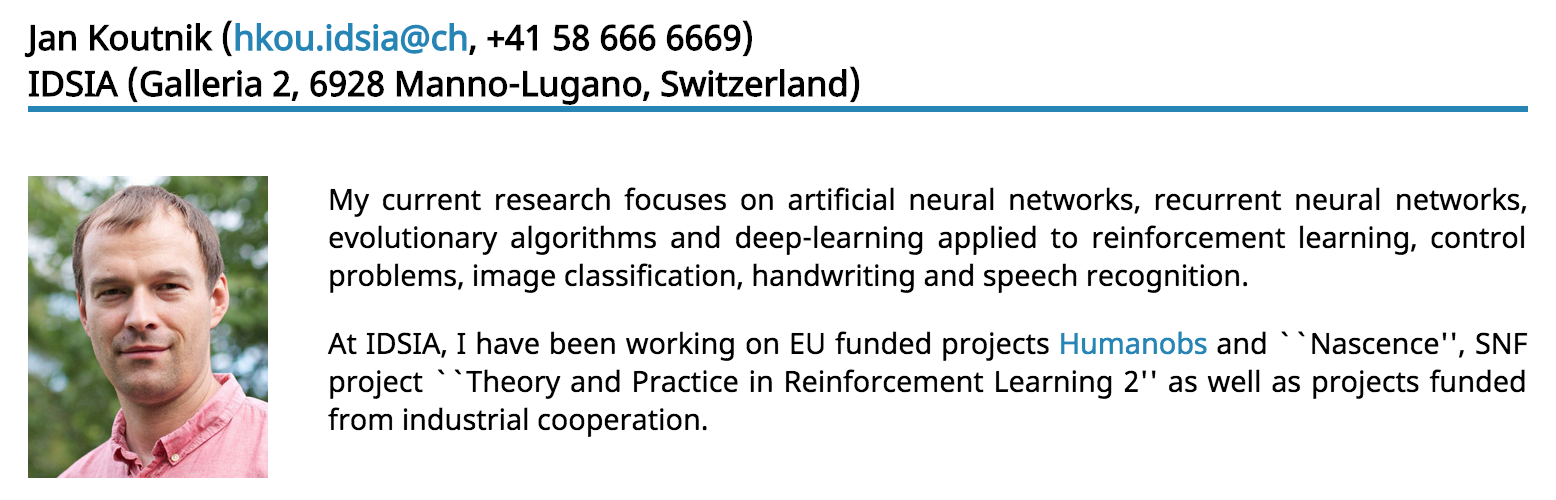
\includegraphics[width=4.1in]{Images/author.png}   
		\end{center}   
		\caption{Main author - Jan Koutnik}
	\end{figure}
}
\frame
{
	\frametitle{Contributions}
	\begin{itemize}
        \item Introduce a new RNN structure \textit{Clockwork} RNN (CW-RNN) :
			\begin{enumerate}
			\item Hidden layer is partitioned into separate module
			\item Each processing inputs at its own clock rate
			\end{enumerate}
		\item Contribution points
			\begin{itemize}
			\item CW-RNN reduces the number of RNN parameters
			\item Improve the performance and speed up the network evaluation
            \item Esp., audio signal generation and TIMIT spoken word classification
			\end{itemize}
	\end{itemize}
}
\section{Brief summary to RNN/LSTM}
\frame
{
    \frametitle{RNN summary - Forward pass}
    \begin{columns}[c]
    		\column{.3\textwidth}
		\begin{figure}[ht]  
			\begin{center}
				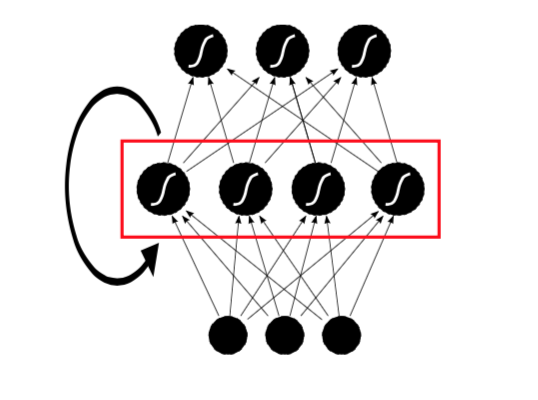
\includegraphics[width=1.6in]{Images/recurrentNN.png}   
			\end{center}   
		\end{figure}
    		\column{.6\textwidth}
			\begin{figure}[ht]  
    			\begin{center}
    				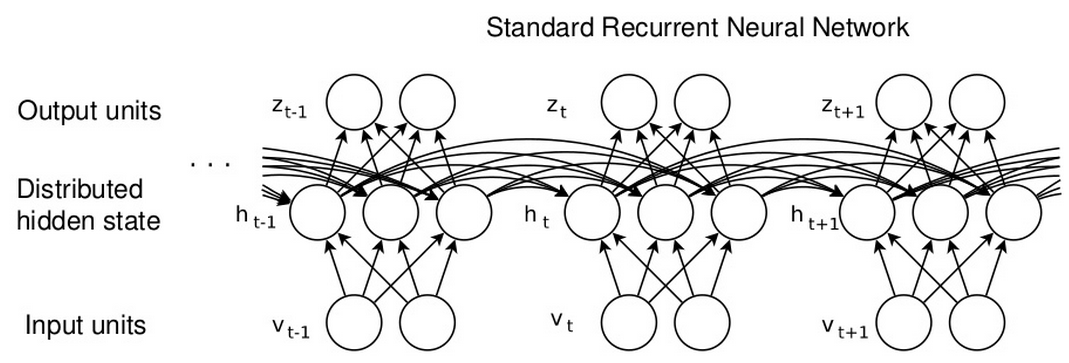
\includegraphics[width=2.6in]{Images/standard_rnn.png}       			
    			\end{center}
    			\end{figure}
	\end{columns}
    \begin{itemize}
        \item Hidden units : 
        $ a_h^t = {\sum_{i=1}^I} W_{ih}x_i^t + \sum_{h'=1}^H w_{h'h} {b_{h'}}^{t-1} $ \\
        Usually initial values $b_i^0$ are chosen to zero / 
        Some cases RNN stability can be improved by using nonzero initial values.
        \item Activaction function :
        $ b_h^t = \theta_h(a_h^t) $
        \item Output units : 
        $ a_k^t = \sum_{h=1}^H w_{hk}b_h^t $
    \end{itemize}
}
\frame
{
    \frametitle{RNN summary - Backward pass \\ Backpropagation through time (BPTT)}
    \begin{itemize}
        \item Like standard backpropagtion, consists of a repeated chain rule (depends on the next $t+1$ state) \\ 
            \vspace{0.1in}
            $ \delta_h^t = \theta'(a_h^t) \Big( \sum_{k=1}^K \delta_k^t w_{hk} + 
            \sum_{h'=1}^H \delta_{h'}^{t+1} w_{hh'} \Big)$ \\
            \vspace{0.1in}
            where $\delta_j^t \equiv \frac{\partial O}{\partial a_j^t} $
        \item Since the weights to and from each unit in the hidden layer are the same at every time step, 
            we need to sum over the whole sequence to get the derivatives : \\
            \vspace{0.1in}
            $ \frac{\partial O}{\partial w_{ij}} = \sum_{t=1}^T \frac{\partial O}{\partial a_j^t} \frac{\partial a_j^t}{\partial w_{ij}} = \sum_{t=1}^T \delta_j^t b_i^t $
    \end{itemize}
}
\frame
{
    \frametitle{BDRNN summary}
	\begin{figure}[ht]  
		\begin{center}
			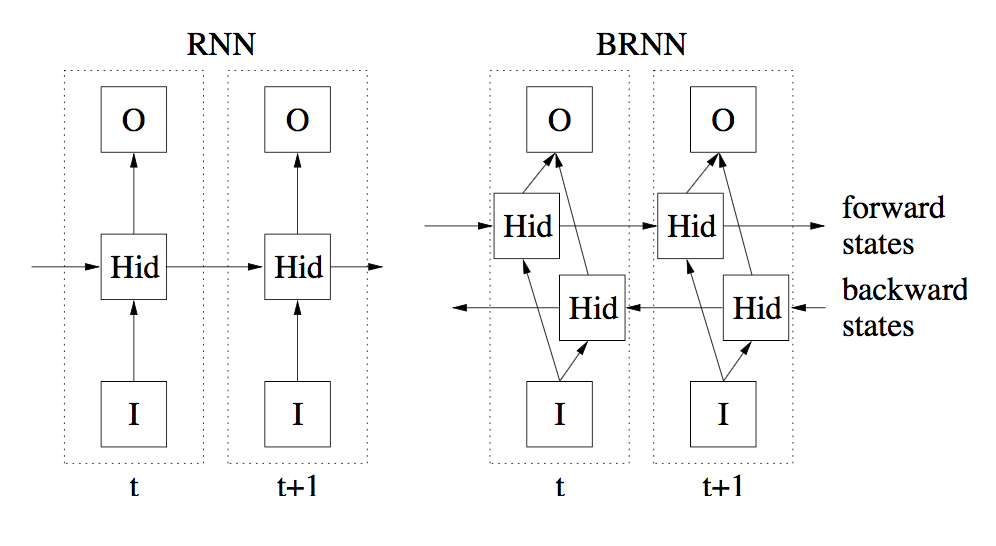
\includegraphics[width=2.2in]{Images/BDRNN_RNN.png}   
		\end{center}   
		\caption{Comparison between BDRNN and RNN}
	\end{figure}
    \begin{itemize}
        \item BDRNN (Bidirectional recurrent neural network) 
        \item Present each training sequence forwards and backwards to two separate recurrent hidden layers, 
            both of which are connected to the same output layer
    \end{itemize}
}
\frame
{
    \begin{itemize}
        \item Forward pass for BDRNN 
            \begin{itemize} 
                \item Generally same as for a undirectional RNN, 
                \item The input sequence is presented in opposite directions to the two hidden layers. 
                \item The output layer is not updated until both hidden layers have processed the entire input sequence:
	            \begin{figure}[ht]  
	            	\begin{center}
	            		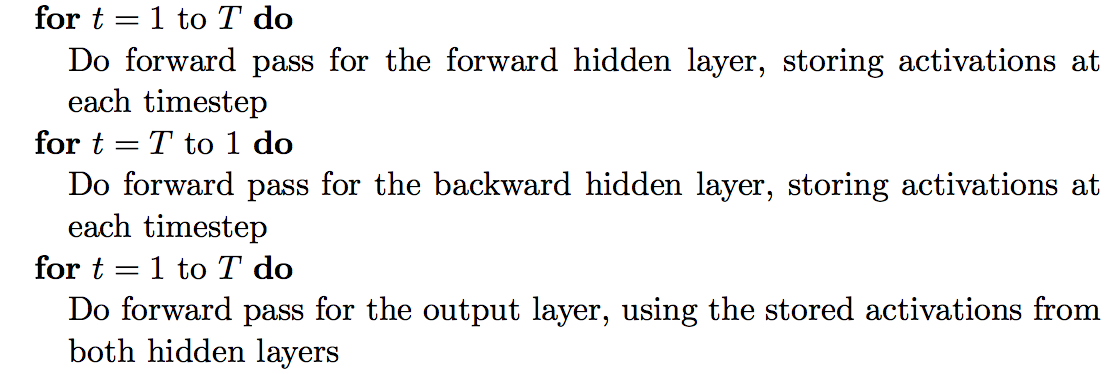
\includegraphics[width=3.5in]{Images/BDRNN_forward_pass.png}   
	            	\end{center}   
	            \end{figure}
            \end{itemize}
    \end{itemize}
}
\frame
{
    \begin{itemize}
        \item Backward pass for BDRNN 
            \begin{itemize} 
                \item Similar to the backward pass proceeds as for a standard RNN training with BPTT  
                \item All the output layer $ \delta $ terms are calculated first, 
                    then fed back to the two hidden layers in opposite directions:
	            \begin{figure}[ht]  
	            	\begin{center}
	            		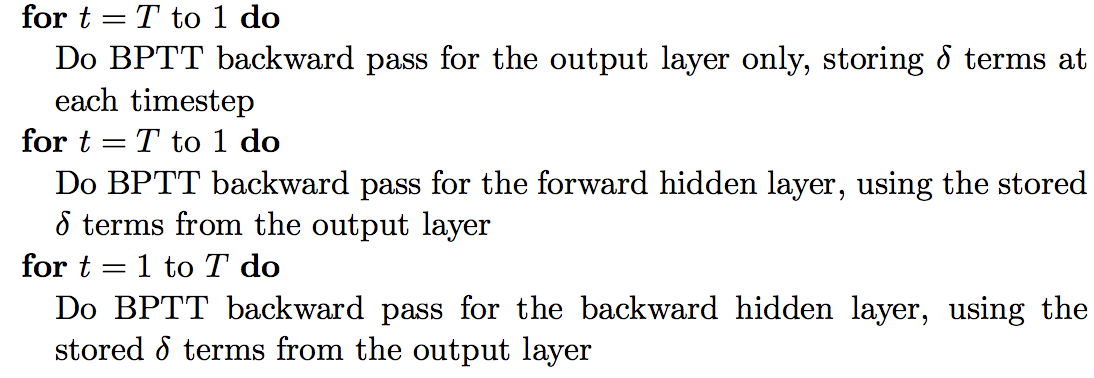
\includegraphics[width=3.5in]{Images/BDRNN_backward_pass.png}   
	            	\end{center}   
	            \end{figure}
            \end{itemize}
    \end{itemize}
}
\frame
{
    \begin{itemize}
        \item BDRNN and Causal tasks 
            \begin{itemize} 
                \item For tasks requiring future inputs, BDRNN cannot be applied (e.g., financial prediction, robot navigation and etc.)  
                \item A task where the input sequences are spatial and not temporal is rightly applicable (e.g., protein prediction)
                \item However, some temporal tasks can also be applied, as long as the network outputs are only needed at the end of some input segment (e.g., speech and handwriting recognition - data is usually divided up into sentences, lines, or dialogue turns and etc.)
            \end{itemize}
    \end{itemize}
}
\frame
{
    \frametitle{LSTM summary}
	\begin{figure}[ht]  
		\begin{center}
			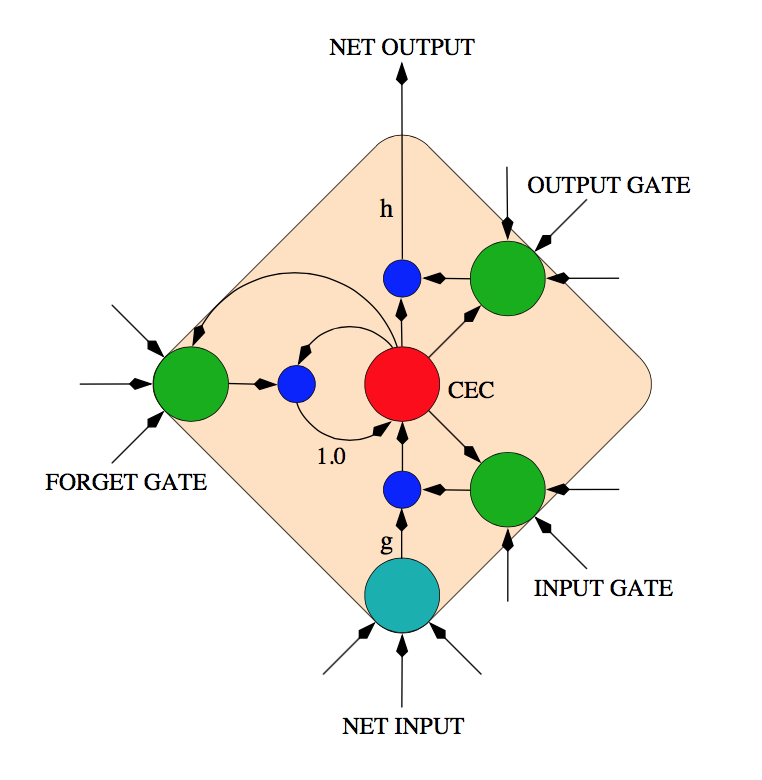
\includegraphics[width=2.2in]{Images/LSTM.png}   
		\end{center}   
		\caption{LSTM structure}
	\end{figure}
}
\frame
{
	\begin{figure}[ht]  
		\begin{center}
			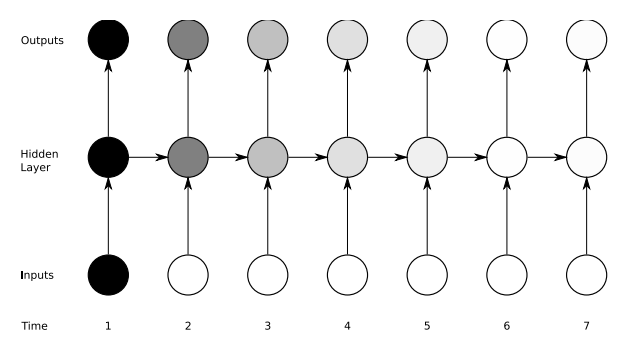
\includegraphics[width=3.2in]{Images/rnn_vanishing_gradients.png}   
		\end{center}   
		\caption{Vanishing gradient problem for RNNs}
	\end{figure}
	\vspace{-0.5cm}
	\begin{itemize}
		\item The sensitivity of the network decays exponentially over time as new inputs overwrite the activation of hidden unit and the network "forgets" the first input. 
	\end{itemize}
}
\frame
{
	\begin{columns}
		\column{0.5\textwidth}
		\begin{figure}[ht]  
			\begin{center}
				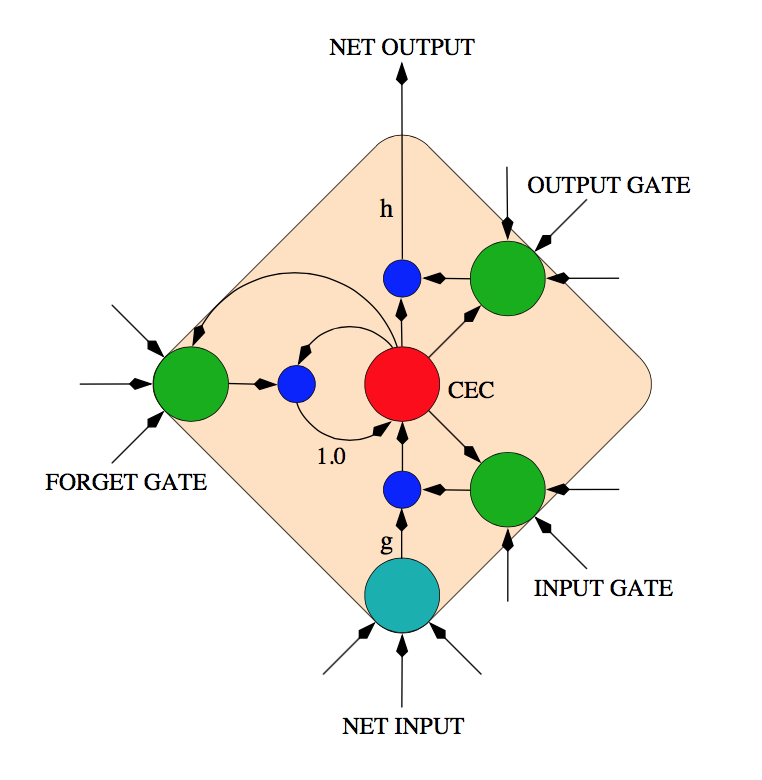
\includegraphics[width=2.1in]{Images/LSTM.png}   
			\end{center}   
			\caption{\centering LSTM memory block with a single cell}
		\end{figure}
		\column{0.6\textwidth} 
		\begin{itemize}
		\item LSTM architecture - consists of a set of memory blocks	
		\item Each block contains one or multiple self-connected memory cells and three multiplicative units	(analogous to memory chips in digital computer)
			\begin{enumerate}
			\item the input gate - write
			\item the output gate - read
			\item the forget gate - reset
			\end{enumerate}
		\end{itemize}
	\end{columns}
}
\frame
{
	\begin{columns}
		\column{0.4\textwidth}
		\begin{figure}[ht]  
			\begin{center}
				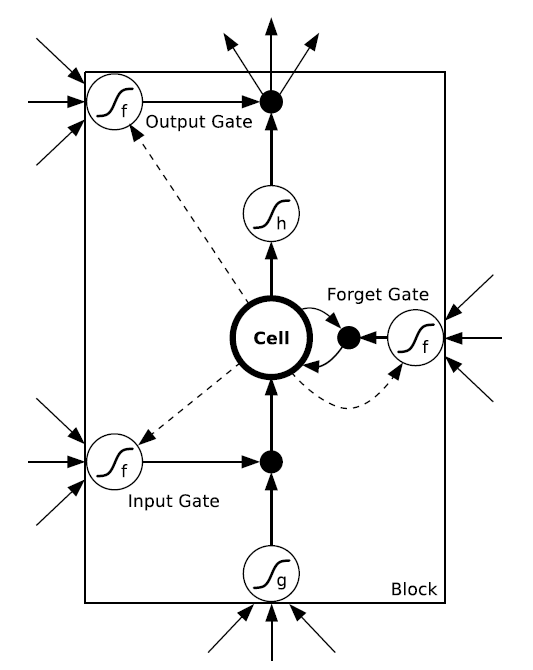
\includegraphics[width=1.8in]{Images/LSTM_detail.png}   
			\end{center}   
			\caption{\centering LSTM memory block with a single cell}
		\end{figure}
		\column{0.7\textwidth} 
		\begin{itemize}
		\item The most important component is the cell has a linear self-loop with forget gate: 
		\begin{itemize}
			\item Self-loop weight is controlled by a forget gate unit ${ f }$
			\item Gated linear self-loop (leaky units or "Constant Error Carousel" (CEC)) helps gradients to be flown for a long durations. (Accumulate information - integration unit over a long duration) 
			\item Using a forget gate, we also can forget the old state of a cell 
		\end{itemize}
		\end{itemize}
	\end{columns}
}
\frame
{
	\begin{columns}
		\column{0.4\textwidth}
		\begin{figure}[ht]  
			\begin{center}
				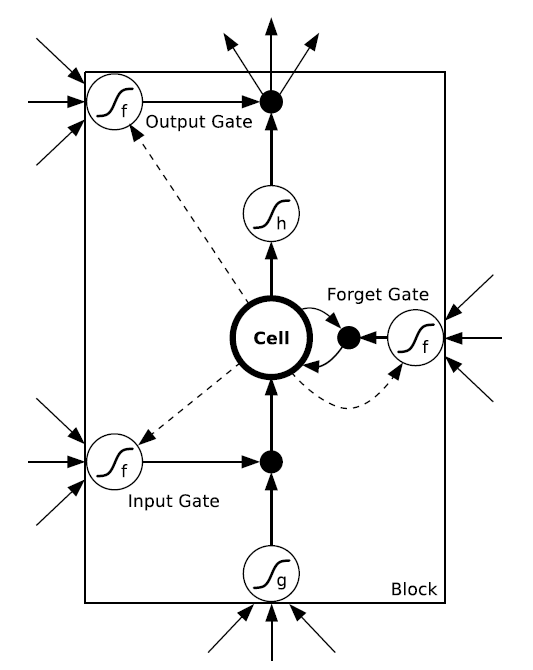
\includegraphics[width=1.8in]{Images/LSTM_detail.png}   
			\end{center}   
			\caption{\centering LSTM memory block with a single cell}
		\end{figure}
		\column{0.7\textwidth} 
		\begin{itemize}
			\item The input and output gates multiply the input and output of the cell via multiplication (small black circles)
			\item Forget gate multiplies the cell's previous state
			\item The gate activation function '${ f }$' is usually the logistic sigmoid
			\item The cell input and output activation functions ('${ g }$' and '${ h }$') are usually tanh or logistic sigmoid
		\end{itemize}
	\end{columns}
}
\frame
{
	\begin{columns}
		\column{0.4\textwidth}
		\begin{figure}[ht]  
			\begin{center}
				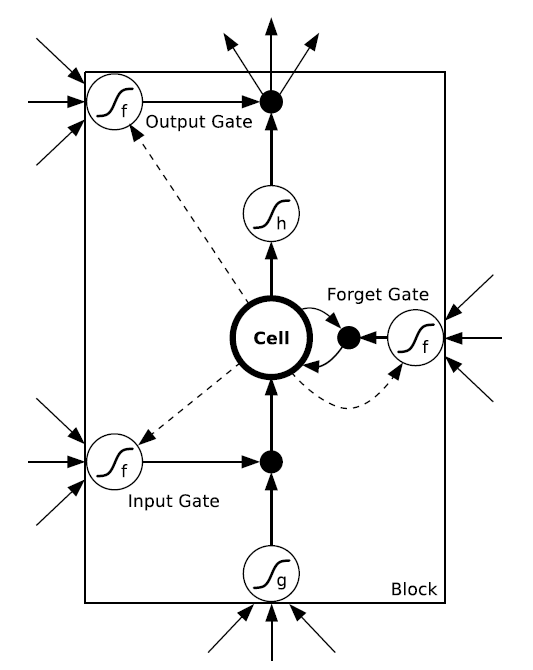
\includegraphics[width=1.8in]{Images/LSTM_detail.png}   
			\end{center}   
			\caption{\centering LSTM memory block with a single cell}
		\end{figure}
		\column{0.7\textwidth} 
		\begin{itemize}
			\item The weighted 'peephole' connections from the cell to the gates are shown as dashed lines
			\begin{itemize}
				\item Peephole connections - weighted connections from the CEC to the gates of the same memory block
				\item If there is no peephole connections, none of the gates has access to the CECs when the output gate is closed. 
			\end{itemize}	
		\end{itemize}
	\end{columns}
}
\frame
{
		\begin{figure}[ht]  
			\begin{center}
				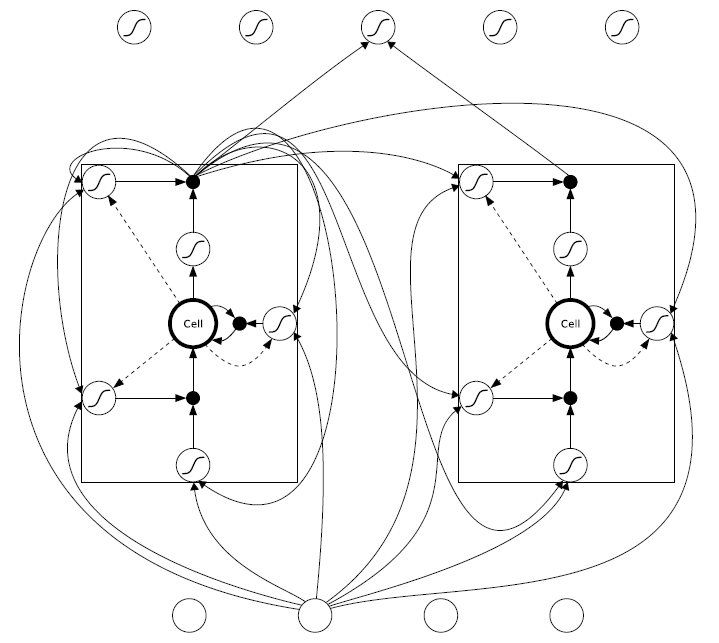
\includegraphics[width=2.6in]{Images/LSTM_network.png}   
			\end{center}   
			\caption{\centering LSTM network consisting of four input units / a hidden layer of two single-cell LSTM memory blocks and five output units}
		\end{figure}
}
\frame
{
		\begin{figure}[ht]  
			\begin{center}
				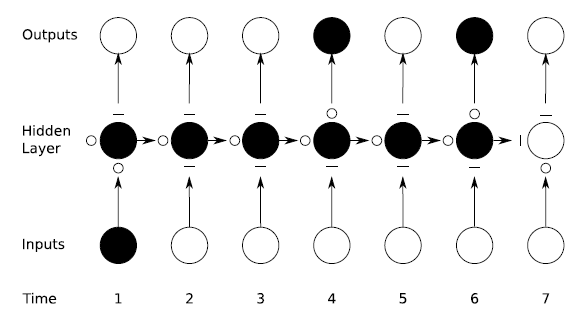
\includegraphics[width=2.6in]{Images/LSTM_preserving_gradient.png}   
			\end{center}   
			\caption{\centering Preservation of gradient information by LSTM}
		\end{figure}
		\vspace{-0.5cm}
		\begin{itemize}
			\item The black nodes - maximally sensitive / white nodes - entirely insensitive
			\item The memory cell remembers the first input as long as the forget gate is open and the input gate is closed
		\end{itemize}
}
\frame
{
  \frametitle{Some comments from Andrew Ng}
   \begin{figure}[ht]  
		\begin{center}
			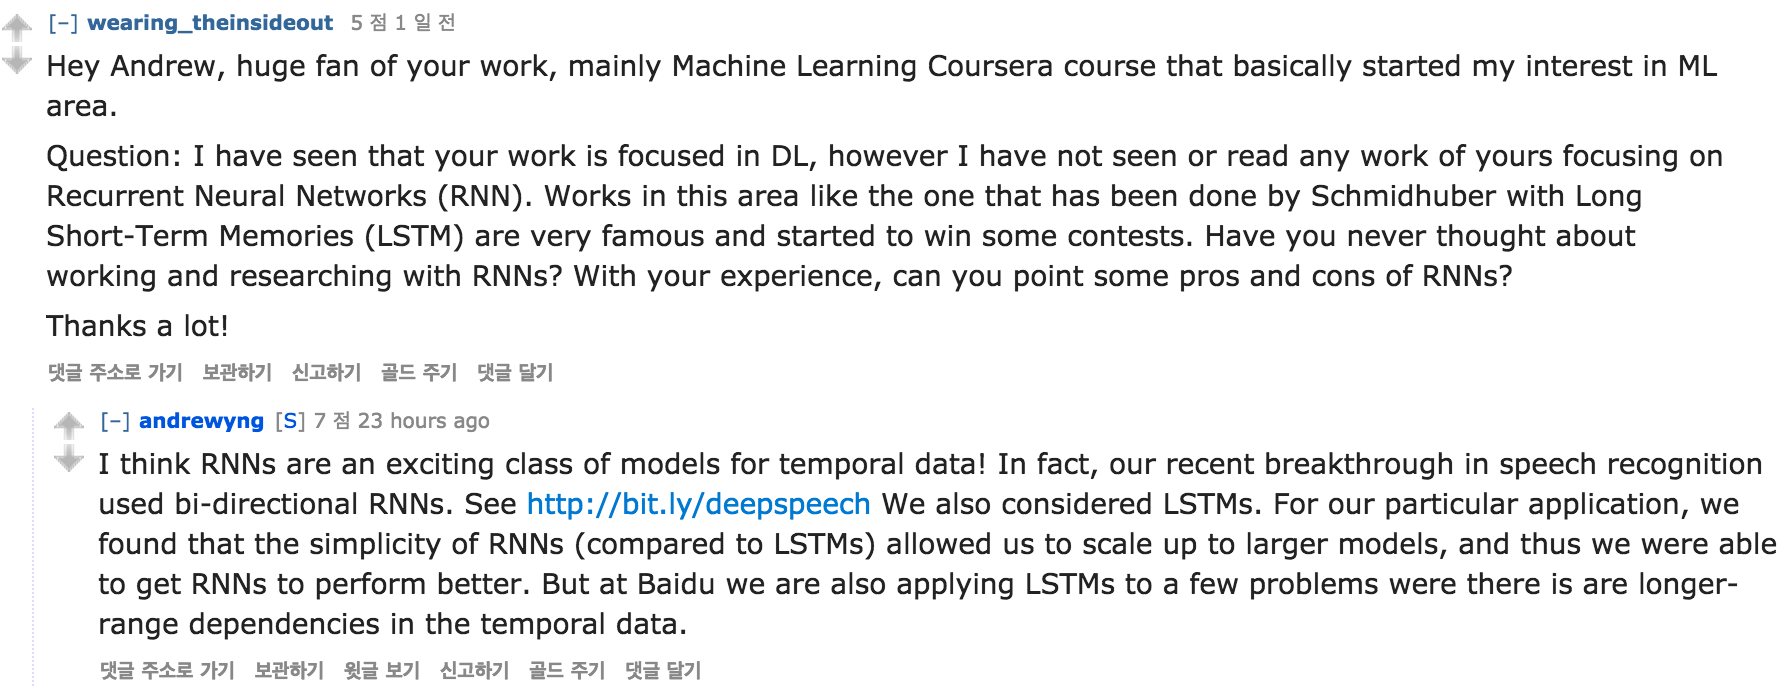
\includegraphics[width=4.5in]{Images/comment_rnn_ng.png}   
		\end{center}   
		\caption{Comments from Andrew Ng of RNN}
	\end{figure}
}
\section{Clockwork RNN (CwRNN)}
\frame
{
   \frametitle{Details of CwRNN}
   \begin{itemize}
   	\item Like standard rnn (SRNN), CwRNN consists of input, hidden and output layers
   	\item Unlike SRNN, the neurons in the hidden layer are partitioned into \textit{g} modules of size k. 
   	\item Each of the modules is assigned a clock period ${T_n \in \{T_1, ..., T_g\} }$ 
   	\item Each module is internally fully-interconnected / recurrent connections from module \textit{j} to module \textit{i} exists only if the period ${T_i}$ is smaller than period ${T_j}$
   \end{itemize}
}
\frame
{
	\begin{figure}[ht]  
		\begin{center}
			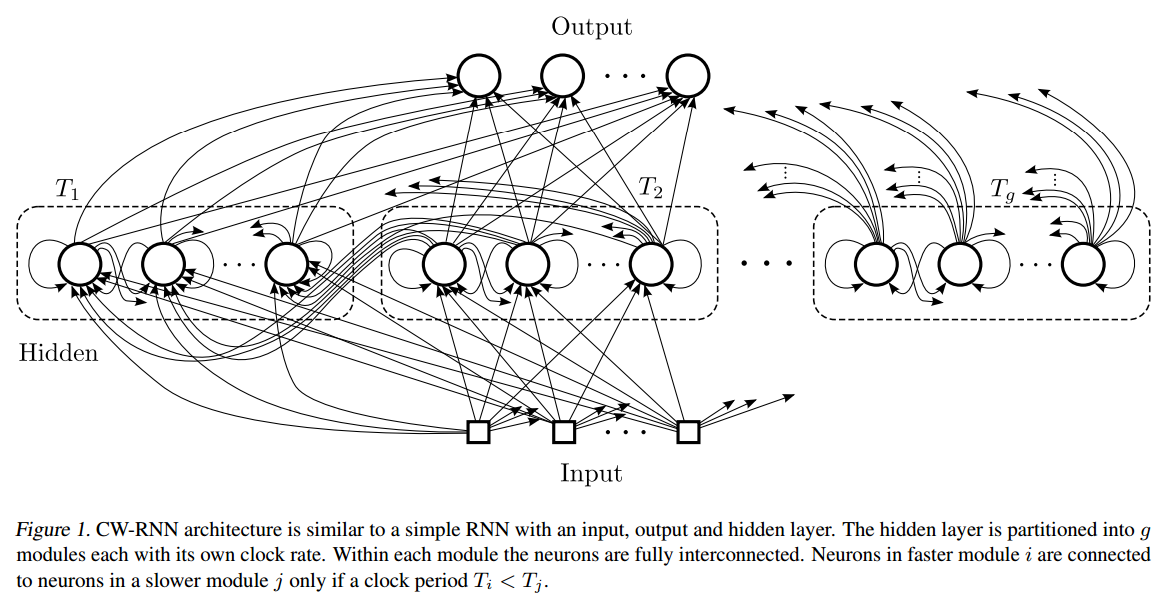
\includegraphics[width=4.1in]{Images/cwrnn.png}   
		\end{center}   
	\end{figure}
   \begin{itemize}
   	\item Sorting the modules by increasing period, connections between modules propagate the hidden state \textit{right-to-left} or \textit{slower to faster} modules.
   \end{itemize}
}
\frame
{
	\begin{figure}[ht]  
		\begin{center}
			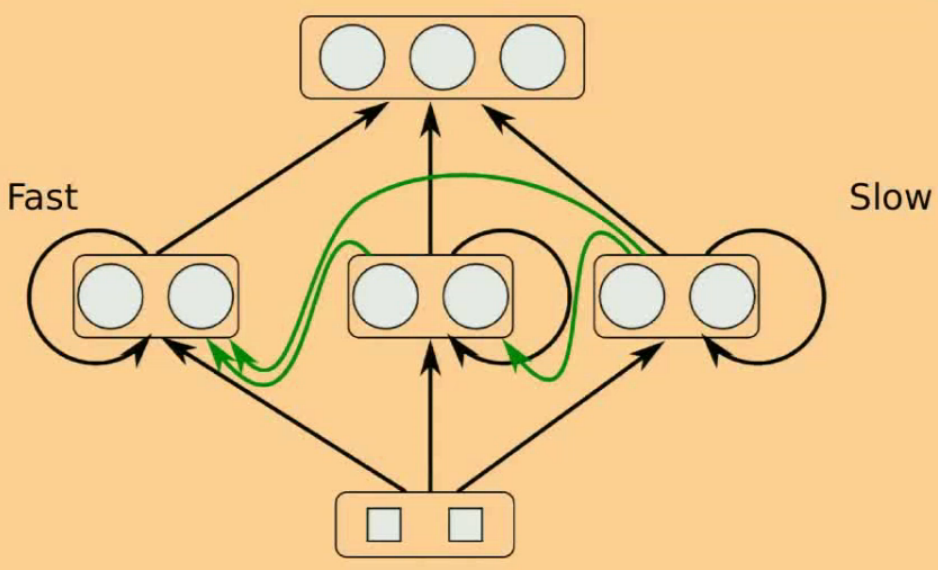
\includegraphics[width=4.1in]{Images/cwrnn_fast_slow.png}   
		\end{center}   
		\caption{Simplified form of CwRNN}
	\end{figure}
}
\frame
{
	\begin{itemize}
		\item In case of CwRNN, only the output of modules ${i}$ satisfying (${t}$ MOD ${T_i}$) = 0 are executed		
		\item In this paper, author uses the exponential series of periods : ${T_i = 2^{i-1} }$
		\item Recall standard RNN output, ${y_O^{(t)}}$, at a time step ${t}$ : \\
		\begin{center}
			${ \mathbf{y}_H^{(t)} = f_H ( \mathbf{W}_H\times \mathbf{y}^{(t-1)} + \mathbf{W}_I\times \mathbf{x}^{(t)}) }$ \\
			${ \mathbf{y}_O^{(t)} = f_O ( \mathbf{W}_O \times \mathbf{y}_H^{(t)} ) }$
		\end{center}			
		\item In case of CwRNN, block-row matrix is used for calculation
	\end{itemize}	
}
\frame
{
	\begin{columns}
	\column{0.5\textwidth}	
	\begin{figure}[ht]  
		\begin{center}
			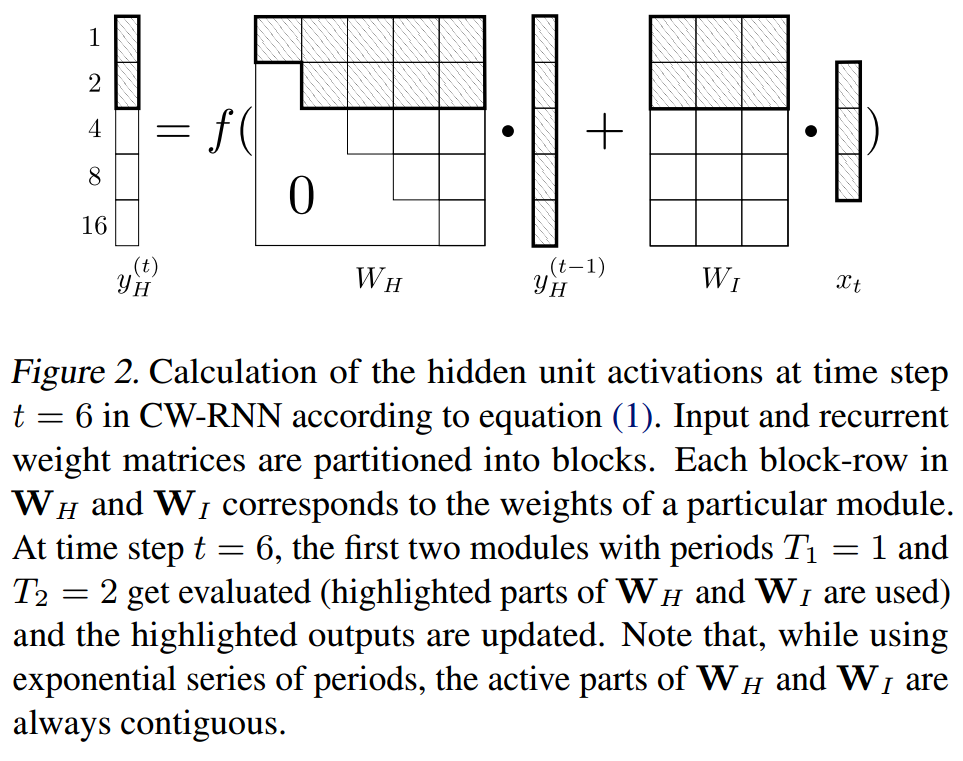
\includegraphics[width=2.1in]{Images/cwrnn_calculation.png}   
		\end{center}   
	\end{figure}	
						
	\column{0.5\textwidth}	
	\begin{itemize}
		\item Matrices ${\mathbf{W}_H}$ and ${\mathbf{W}_I}$ are partitioned into ${g}$ blocks-rows: 
	\end{itemize}	
	\[
	\mathbf{W}_H=
  \begin{bmatrix}
    \mathbf{W}_{H_1} \\
    \vdots \\
    \mathbf{W}_{H_g} 
  \end{bmatrix}
  %
  \hspace{0.5cm}
  %
  \mathbf{W}_I=
  \begin{bmatrix}
    \mathbf{W}_{I_1} \\
    \vdots \\
    \mathbf{W}_{I_g} 
  \end{bmatrix}
\]
  	\begin{itemize}
  		\item ${ \mathbf{W}_H }$ is a block-upper triangular matrix
  	\end{itemize}
  	
	\end{columns}
}
\frame
{
   \frametitle{Experiments}
   \begin{itemize}
   	\item Experimental setup
   		\begin{itemize}
   			\item Compared to the simple RNN (SRNN) and LSTM networks
   			\item All networks have one hidden layer with the \textit{tanh} activation function
   			\item Number of nodes in the hidden layer was chosen to obtain the same number of parameters for all three methods   			
   			\item Initial values for all weights were drawn from a Gaussian distribution with zero mean with std 0.1
   			\item Trained with SGD with Nesterov-style momentum
   		\end{itemize}
   \end{itemize}
}
\frame
{
   \frametitle{Experiments - Sequence Generation}
   \begin{columns}
		\column{0.4\textwidth}
		\begin{figure}[ht]  
			\begin{center}
				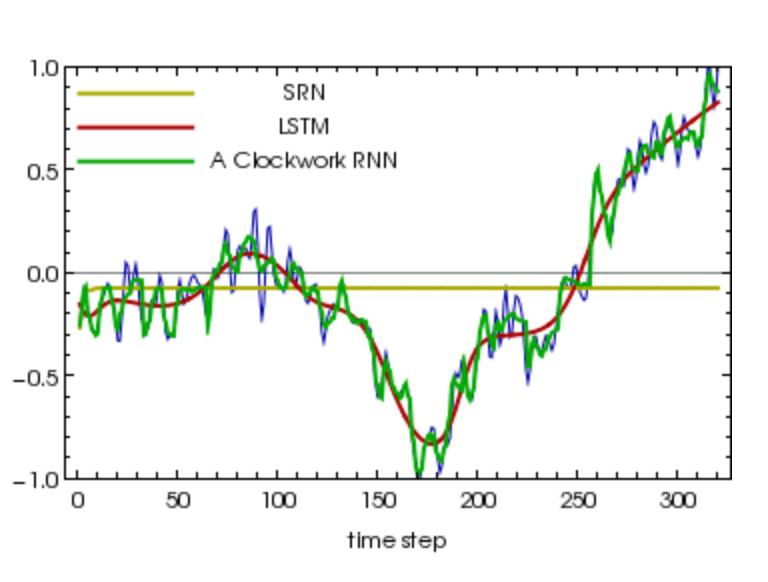
\includegraphics[width=1.8in]{Images/cwrnn_graph.png}   
			\end{center}   
			\caption{\centering Sequence generation examples}
		\end{figure}
		\column{0.7\textwidth} 
		\begin{itemize}		
			\item The goal of this task - Generate a target sequence as accurately as possible
			\item Five different target sequences were created - sampling a piece of music at 44.1Hz for 7ms
			\item Resulting sequences were scaled to the interval [-1, 1]
			\item All networks were trained over 2000 epochs
			\item ${3\times10^{-1}}$ optimal for RNN/CwRNN and ${3\times10^{-5}}$ for LSTM
		\end{itemize}
	\end{columns}
}
\frame
{
	\begin{figure}[ht]  
		\begin{center}
			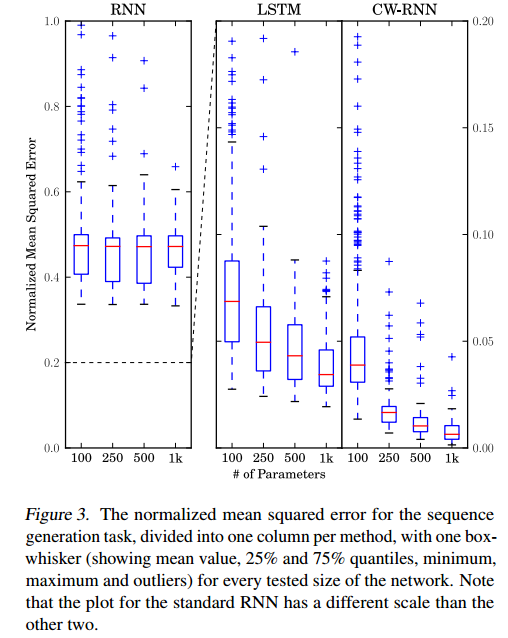
\includegraphics[width=2.3in]{Images/cwrnn_sequence_result.png}   
		\end{center}   
	\end{figure}
}
\frame
{
	\begin{figure}[ht]  
		\begin{center}
			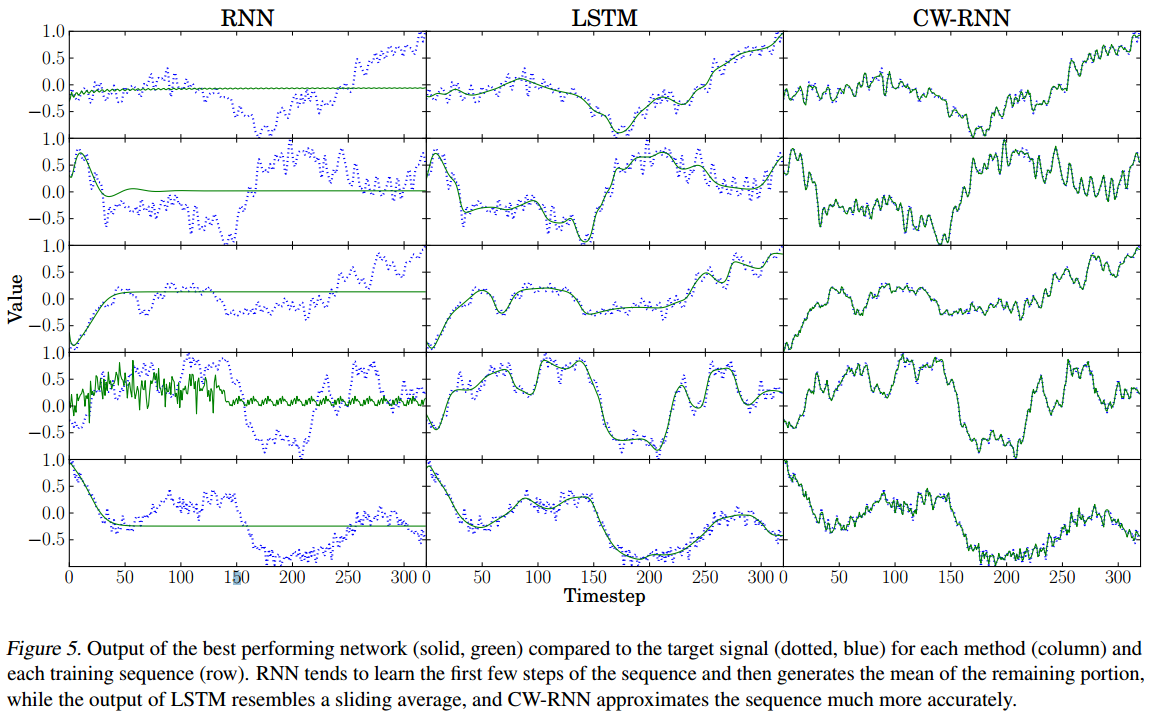
\includegraphics[width=4.3in]{Images/cwrnn_output.png}   
		\end{center}   
	\end{figure}
}
\frame
{
   \frametitle{Experiments - Spoken Word Classification}
   \begin{columns}
		\column{0.55\textwidth}
		\begin{itemize}		
			\item Sequence classification containing an audio signal of one spoken word from the TIMIT dataset  
			\item Dataset contains 25 different words arranged in 5 clusters based on their suffix 
			\item Because of the suffix-similarity, network needs to learn long-term dependencies
			\item 12 dimensional MFCC vector plus energy, 13 channels normalized			
		\end{itemize}
		\column{0.55\textwidth} 
		\begin{itemize}
			\item \textbf{Cluster 1:} making, walking, cooking, looking, working
			\item \textbf{Cluster 2:} biblical, cyclical, technical, classical, critical
			\item \textbf{Cluster 3:} tradition, addition, audition, recognition, competition
			\item \textbf{Cluster 4:} musicians, discussions, regulations, accusations, conditions
			\item \textbf{Cluster 5:} subway, leeway, freeway, highway, hallway
		\end{itemize}		
	\end{columns}
}
\frame
{
	\begin{figure}[ht]  
		\begin{center}
			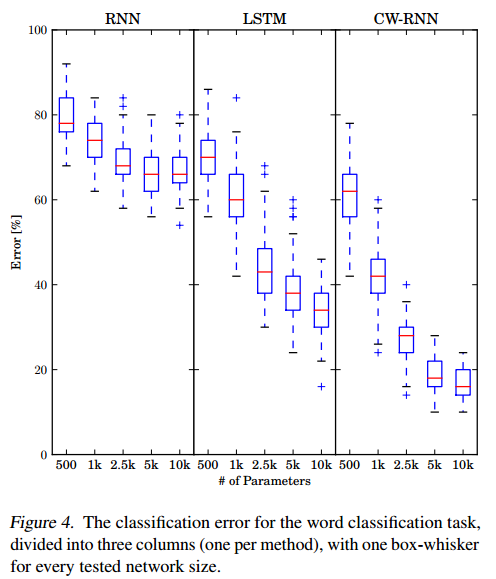
\includegraphics[width=2.5in]{Images/cwrnn_word_classification.png}   
		\end{center}   
	\end{figure}
}
\frame
{
   \frametitle{Experiments - Online Handwritten Recognition}
   \begin{figure}[ht]  
			\begin{center}
				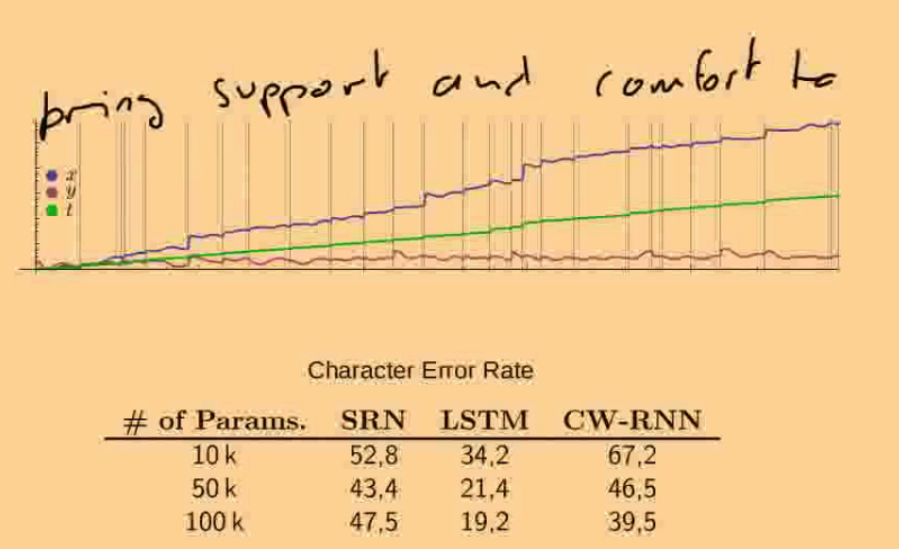
\includegraphics[width=3.8in]{Images/cwrnn_handwritten.png}   
			\end{center}   
			\caption{\centering Sequence generation examples}
	\end{figure}
}
\frame
{
   \frametitle{Some comments from Schmidhuber}
   \begin{figure}[ht]  
		\begin{center}
			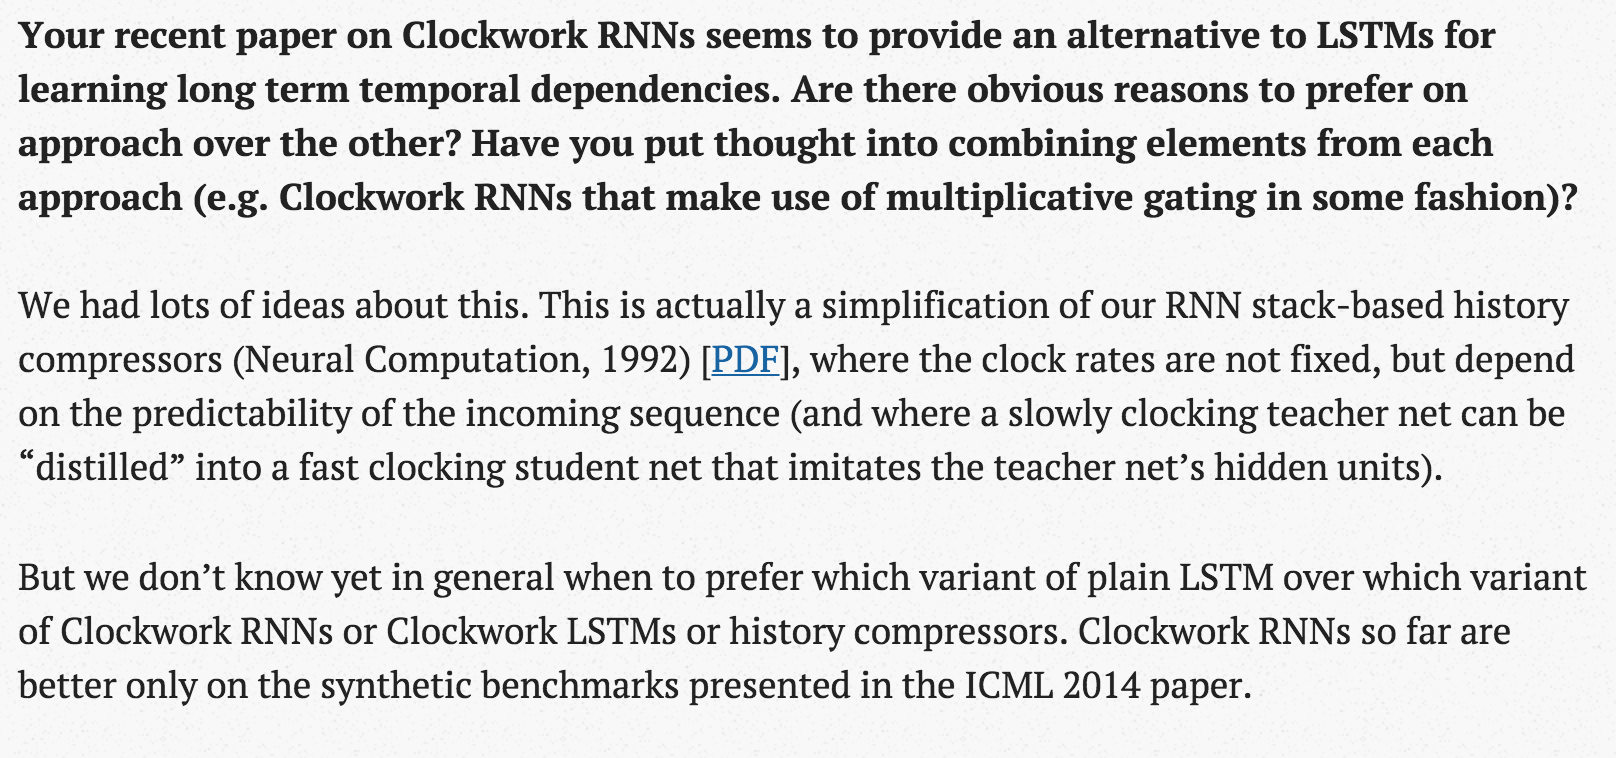
\includegraphics[width=4.2in]{Images/comment_cwrnn.png}   
		\end{center}   
		\caption{Comments from Schmidhuber of Clockwork RNN}
	\end{figure}
}
\frame
{
   \frametitle{Discussion}
   \begin{itemize}
   	\item A simple mechanism to improve modeling of different time-scales
   	\item Superior performance on sequence generation and classification
   	\item Performance in Online handwriting recognition is in-between SRN and LSTM
   	\item Module timings are not flexible enough for handwriting recognition
   \end{itemize}
}
\end{document}